\documentclass[uplatex, dvipdfmx, a4paper, report, papersize, 11pt]{jsbook}
\usepackage{bm}
\usepackage{amsmath}
\usepackage[dvipdfmx]{graphicx}
\usepackage{wrapfig}
\usepackage[hang, small, bf]{caption}
\usepackage[subrefformat=parens]{subcaption}
\usepackage{comment}
\captionsetup{compatibility=false}

\bibliographystyle{jplain}
\title{二色の光周波数コムによるレーザー冷却法の開拓}
\author{物理工学科4年 中西亮}
\date{2018/11/19}
\begin{document}
\maketitle
\newpage

\setcounter{tocdepth}{2}
\tableofcontents


\newpage
\chapter{序論}
\newpage
\begin{figure}[t]
  \centering
    \begin{tabular}{c}
      \begin{minipage}{1\hsize}
        \centering
          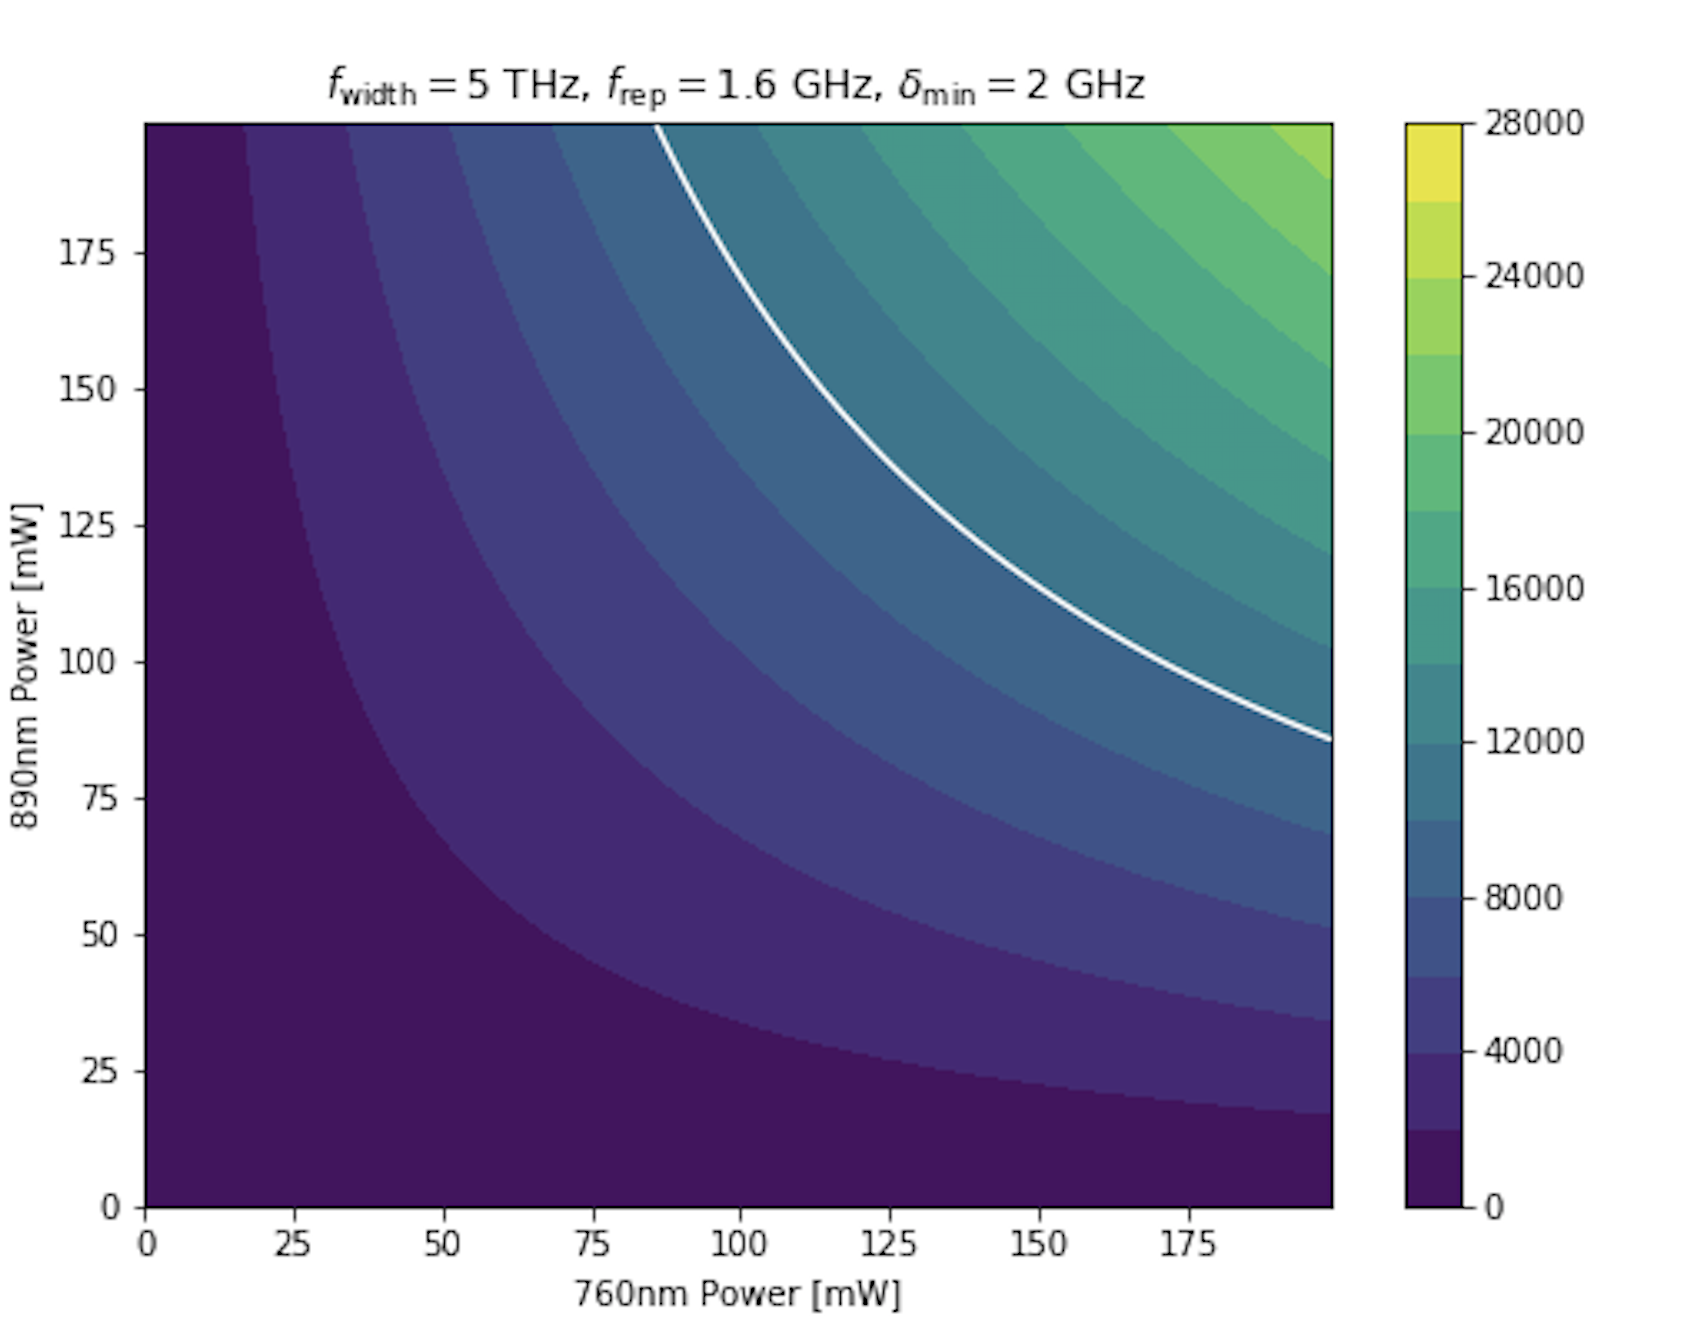
\includegraphics[keepaspectratio,  scale=0.5,  angle=0]
                          {figures/chapter3/5THz-1.6GHz-2GHz_200mW-copy.png}
                          \caption{}
                          \label{5THz-1.6GHz-2GHz_1W}
      \end{minipage}
    \end{tabular}
\end{figure}
\end{document}
